\chapter{Sistemi Multi-Cellulari}
In questo capitolo cercheremo di spiegare cosa accade nella realtà in presenza di sistemi in cui sono presenti diverse celle.
\begin{center}
    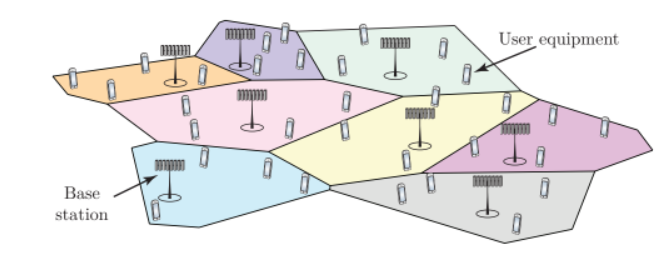
\includegraphics[width=0.8\textwidth]{Images/Accass.png}
\end{center}
Ora con K indicheremo il numero TOTALE di utenti e con $K_b$ l'insieme di utenti serviti dalla BS b.
\section{Sistemi Multi-Cellulari: Uplink}
Definiamo con $\vc{h}_{k,b}$ il vettore di canale tra l'utente k e la BS b, che riceverà il seguente segnale:
\begin{equation*}
    \begin{aligned}
    \vc{r}_b &= \underbrace{\sqrt{p_m} \vc{h}_{m,b}s_m}_{\text{Segnale Utile}} + \underbrace{\sum_{k \in K_b, k \neq m} \sqrt{p_k} \vc{h}_{k,b}s_k}_{\text{Interferenza multi-utente nella cella}} +\\ \\
    &+ \underbrace{\sum_{k \cancel{\in} K_b} \sqrt{p_k} \vc{h}_{k,b}s_k}_{\text{Interferenza multi-utente fuori cella}} + \underbrace{\vc{n}_b}_{\text{Rumore Termico}}
     \end{aligned}
\end{equation*}
Se filtriamo con $\vc{c}_m$ avremo:
\begin{equation*}
\begin{aligned}
        y_b &= \vc{c}_m^H \vc{r}_b = \underbrace{\sqrt{p_m}\vc{c}_m^H \vc{h}_{m,b}s_m}_{\text{Segnale Utile}} + \underbrace{\sum_{k \in K_b, k \neq m} \sqrt{p_k}\vc{c}_m^H \vc{h}_{k,b}s_k}_{\text{Interferenza multi-utente nella cella}} +\\ \\
        &+ \underbrace{\sum_{k \cancel{\in} K_b} \sqrt{p_k}\vc{c}_m^H \vc{h}_{k,b}s_k}_{\text{Interferenza multi-utente fuori cella}} + \underbrace{\vc{c}_m^H\vc{n}_b}_{\text{Rumore Termico}}
\end{aligned}
\end{equation*}
Ora calcoliamo il SINR dell'm-esimo utente:
\begin{equation*}
    SINR_m = \frac{p_m |\vc{c}_m^H\vc{h}_{m,b}|^2}{\sum_{k \in K_b, k \neq m} p_k |\vc{c}_k^H\vc{h}_{k,b}|^2 + \sum_{k \cancel{\in} K_b}  p_k |\vc{c}_k^H\vc{h}_{k,b}|^2 + \sigma^2 ||\vc{c}_m||^2} 
\end{equation*}


\section{Sistemi Multi-Cellulari: Downlink}
Sia $\vc{g}_{m,a}$, il Vettore di Canale tra la BS che chiameremo A, e l'utente m, che riceverà il seguente segnale:
\begin{equation*}
    \begin{aligned}
    \vc{r}_m &= \underbrace{\sqrt{p_m} \vc{g}_{m,A}^H\vc{q}_m s_m}_{\text{Segnale Utile}} + \underbrace{\sum_{k \in K_A, k \neq m} \sqrt{p_k} \vc{g}_{m,A}^H \vc{q}_k s_k}_{\text{Interferenza multi-utente nella cella}} +\\ \\
    &+ \underbrace{\sum_{b \cancel{\in} A} \vc{g}_{m,b}^H \sum_{k \in K_b} \sqrt{p_k} \vc{q}_k s_k}_{\text{Interferenza multi-utente fuori cella}} + \underbrace{\vc{n}_m}_{\text{Rumore Termico}}
     \end{aligned}
\end{equation*}
Che possiamo riscrivere come:
\begin{equation*}
    \begin{aligned}
    \vc{r}_m &= \underbrace{\sqrt{p_m} \vc{g}_{m,A}^H\vc{q}_m s_m}_{\text{Segnale Utile}} + \underbrace{\sum_{k \in K_A, k \neq m} \sqrt{p_k} \vc{g}_{m,A}^H\vc{q}_k s_k}_{\text{Interferenza multi-utente nella cella}} +\\ \\
    &+ \underbrace{\sum_{b \cancel{\in} A} \sum_{k \in K_b}   \sqrt{p_k} \vc{g}_{m,b}^H \vc{q}_k s_k}_{\text{Interferenza multi-utente fuori cella}} + \underbrace{\vc{n}_m}_{\text{Rumore Termico}}
     \end{aligned}
\end{equation*}

Che di conseguenza associa all'utente m il seguente SINR:
\begin{equation*}
    SINR_m = \frac{p_m |\vc{g}_m^H\vc{q}_{m,a}|^2}{\sum_{k \in K_a, k \neq m} p_k |\vc{g}_{m,a}^H\vc{q}_{k}|^2 + \sum_{k \cancel{\in} K_a}  p_k |\vc{g}_{m,b}^H\vc{q}_{k}|^2 + \sigma^2 } 
\end{equation*}
Come possiamo vedere, il modello di segnale è simile al caso di singola cella, quindi possiamo usare le tecniche a noi note (MRT/MRC, ZF, MMSE).